
%(BEGIN_QUESTION)
% Copyright 2006, Tony R. Kuphaldt, released under the Creative Commons Attribution License (v 1.0)
% This means you may do almost anything with this work of mine, so long as you give me proper credit

Her vises et standard trykkmåler, basert på trykkføling i et hul, C-formet metallror kalt et \textit{bourdon-rør}:

$$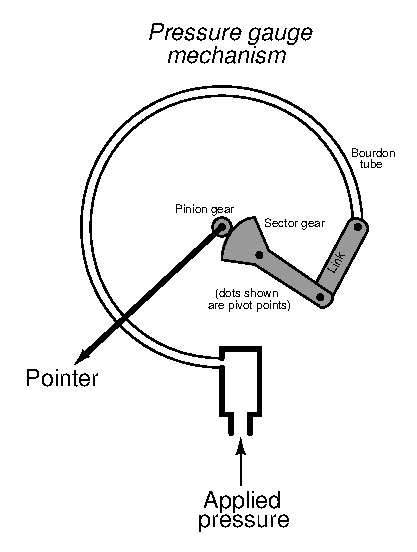
\includegraphics[width=15.5cm]{i00173x01.eps}$$

Bruk piler og spor bevegelsene til alle bevegelige deler i denne mekanismen når trykket som pålegges tilkoblingen nederst på bourdon-røret øker.

\vskip 10pt

Beskriv også hvordan måleområdet til dette trykkmåleret kan endres.  Med andre ord: hva må flyttes, justeres eller endres i mekanismen for å endre forholdet mellom pålagt trykk og viserbevegelse?

\vskip 20pt \vbox{\hrule \hbox{\strut \vrule{} {\bf Suggestions for Socratic discussion} \vrule} \hrule}

\begin{itemize}
\item{} Spørsmål som dette er ofte krevende for personer med begrenset erfaring med mekaniske innretninger.  Identifiser noen problemlosingsstrategier en mekanisk uerfaren student kan bruke på slike oppgaver.
\item{} Hvilket utstyr ville du foresla å bruke for å pålegge et nøyaktig kjent trykk på et manometer for kalibrering?
\item{} Anta at et trykkmåler skal brukes i en prosess der det måler væsketrykk.  Er det greit å kalibrere det på testbenk med komprimert \textit{luft} i stedet for væsken som brukes i felt?  Hvorfor eller hvorfor ikke?
\end{itemize}

\underbar{file i00173}
%(END_QUESTION)





%(BEGIN_ANSWER)

Delene i denne manometermekanismen vil bevege seg slik:

$$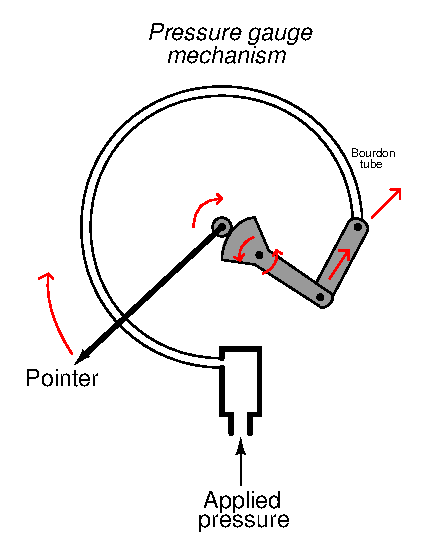
\includegraphics[width=15.5cm]{i00173x02.eps}$$

Mulige endringer for å gjøre denne trykkmålemekanismen mer følsom:

\begin{itemize}
\item{} Reduser fjærkonstanten (``stivheten'') i bourdon-røret
\item{} Forkort armen på sektorhjulet (delen til høyre for pivotpunktet, koblet til linken)
\item{} Øk radius på sektorhjulet
\item{} Reduser radius på pinjonghjulet
\end{itemize}

%(END_ANSWER)





%(BEGIN_NOTES)

Når spissen av bourdon-røret beveger seg opp og til høyre, trekker den i linken og flytter høyre ende av sektoren opp.  Dette roterer sektorhjulet mot klokka rundt pivotpunktet, som igjen roterer pinjonghjulet med klokka.  Denne med-klokka-bevegelsen driver viseren med klokka oppover trykkskalaen (ikke vist).

Jeg anbefaler sterkt å ta med et bourdon-rørs trykkmåler til undervisning for inspeksjon.  Enda bedre er et trykkmåler montert på en deadweight-tester, slik at studentene kan se mekanismen i drift mens trykket økes og reduseres.

\vskip 10pt

Wika har en god YouTube-video som viser produksjon og testing av bourdon-rørs trykkmåler, og den er verdt å vise i klassen.

%INDEX% Measurement, pressure: bourdon tube

%(END_NOTES)
